\documentclass{article}
\usepackage{graphicx} % Required for inserting images
\usepackage{listings}

\title{Oblig 2 TEK5010}
\author{Ada Hatland}
\date{November 2024}

\begin{document}

\maketitle

\section{}
See figure \ref{fig:auction}

\begin{figure}
	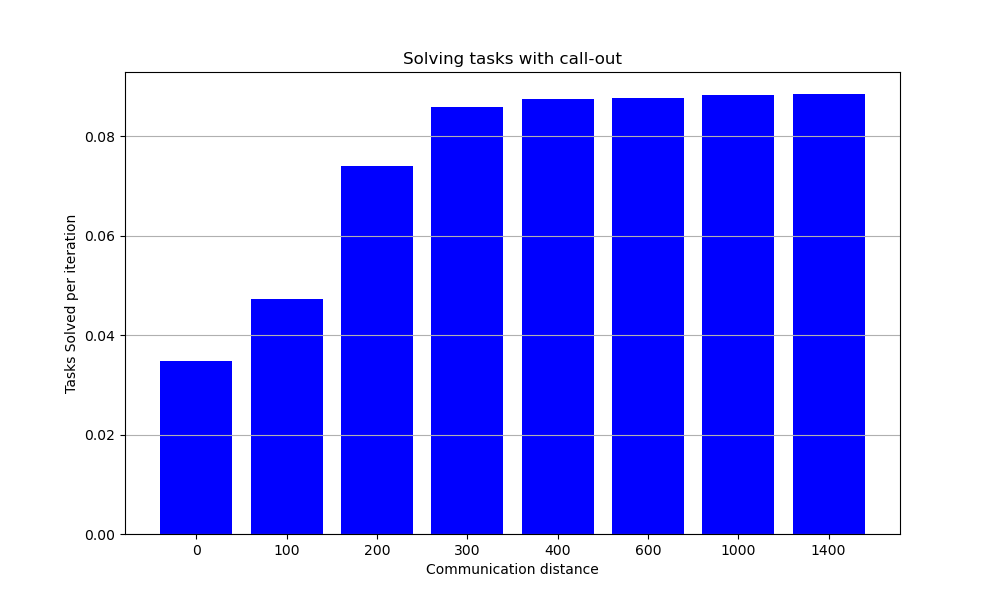
\includegraphics[width=\textwidth]{auction.png}
	\caption{Solving tasks with auction, $T=2$, $T_r=50$, $T_c=3$, $R=30$, 100000 iterations}
	\label{fig:auction}
\end{figure}


\section{}
When we include an auction and only call-out to the closest amount of necessary agents to complete a task we see that after reaching a search range of 300 we get diminishing returns. This implies in the vast majority of cases we find 2 agents within 300 range.

Without the auction, returns decrease after 300, this is because after 300 we more often than not call out to unnecessarily many agents. With the modification of the auction we ensure to never call more agents than necessary, which slightly improve performance for lower ranges, and makes a major difference for high ranges.

See figure \ref{fig:search}

\begin{figure}
	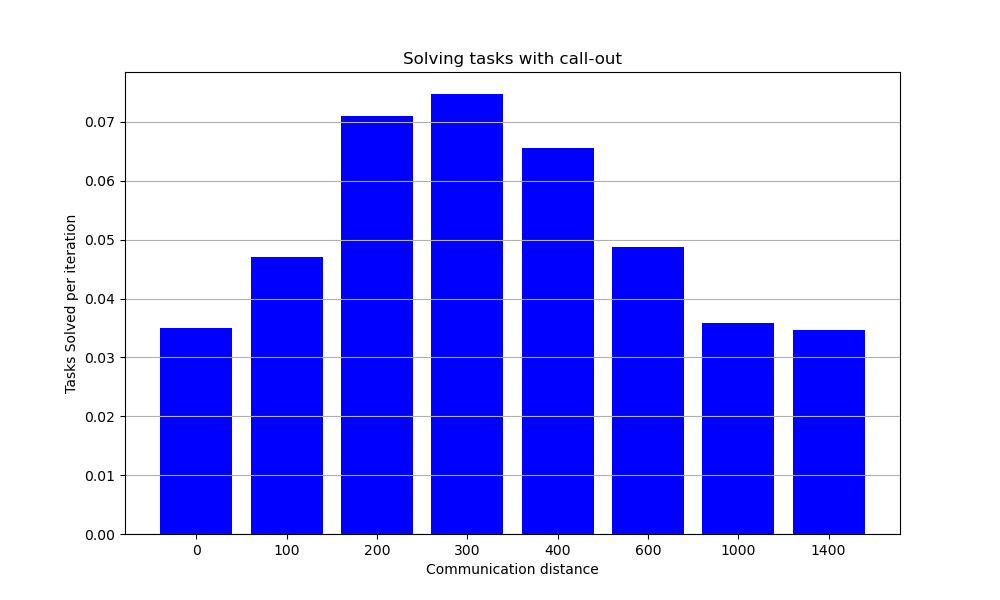
\includegraphics[width=\textwidth]{search_ranges.png}
	\caption{Solving tasks without auction, $T=2$, $T_r=50$, $T_c=3$, $R=30$, 100000 iterations}
	\label{fig:search}
\end{figure}


\section{Comparison between interactive and reactive}
To compare similar cost of reactive and interactive robots we compare simulations of calling out with and without auction, with twice as many robots in the simulation without auction to make up for the cost difference. With a search range of 300, which is when the reactive robots performed the best in our experiment they perform better at least up to 70/140 robots. It looks like tasks solved is proportional to amount of interactive agents but seems to decrease rapidly and then taper off with reactive ones. With a search range of 600 which was suboptimal for the reactive agents it makes a big difference for more than just a few robots. In conclusion, both reactive and interactive robots could perform better depending on the scenario. See figure \ref{fig:comarison} and \ref{fig:comparison2}

\begin{figure}
	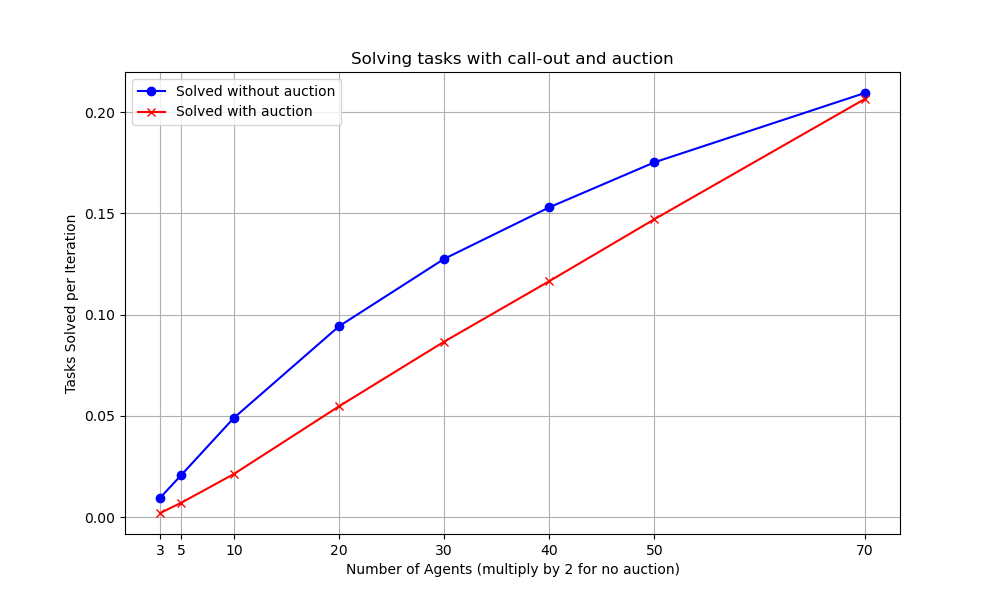
\includegraphics[width=\textwidth]{search_ranges_comparison.png}
	\caption{Solving tasks with and without auction, $T=2$, $T_r=50$, $T_c=3$, $R_d = 300$, 100000 iterations}
	\label{fig:comparison}
\end{figure}


\begin{figure}
	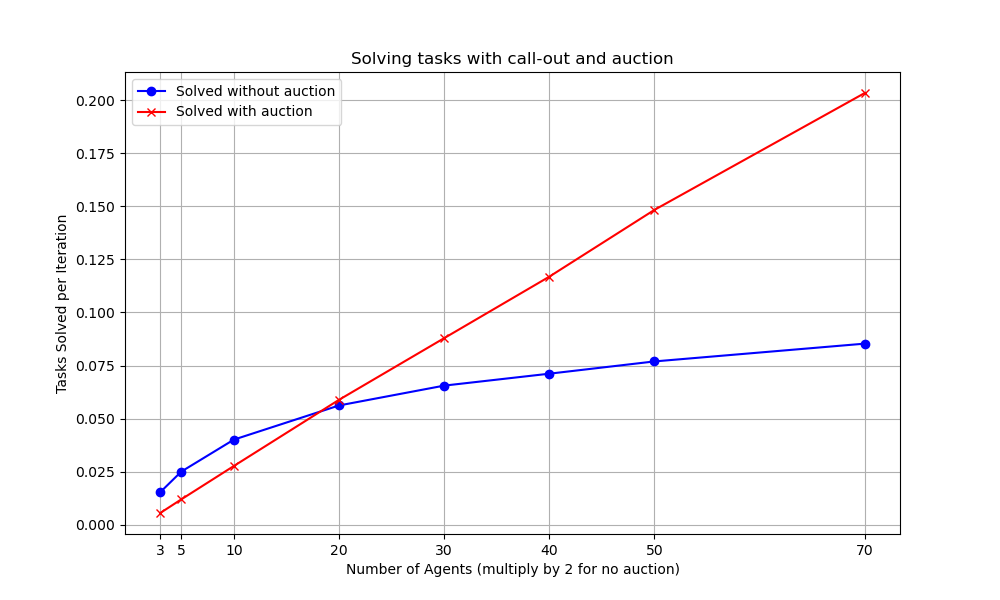
\includegraphics[width=\textwidth]{search_ranges_comparison2.png}
	\caption{Solving tasks with and without auction, $T=2$, $T_r=50$, $T_c=3$, $R_d = 600$, 100000 iterations}
	\label{fig:comparison2}
\end{figure}

\appendix

\section{Agent and task classes}
\lstinputlisting[language=Python]{agent.py}


\section{Simulation code}
\lstinputlisting[language=Python]{main.py}

\end{document}

